% !TeX document-id = {f19fb972-db1f-447e-9d78-531139c30778}
% !BIB program = biber

%\documentclass[handout]{beamer}
\documentclass[compress]{beamer}
\usepackage[T1]{fontenc}
\usetheme[block=fill,subsectionpage=progressbar,sectionpage=progressbar]{metropolis} 
\usepackage{graphicx}

\usepackage{wasysym}
\usepackage{etoolbox}
\usepackage[utf8]{inputenc}

\usepackage{pifont}

\usepackage{threeparttable}
\usepackage{subcaption}

\usepackage{tikz-qtree}
\usepackage{neuralnetwork}

\setbeamercovered{still covered={\opaqueness<1->{5}},again covered={\opaqueness<1->{100}}}


\usepackage{listings}

\lstset{
	basicstyle=\scriptsize\ttfamily,
	columns=flexible,
	breaklines=true,
	numbers=left,
	%stepsize=1,
	numberstyle=\tiny,
	backgroundcolor=\color[rgb]{0.85,0.90,1}
}



\lstnewenvironment{lstlistingoutput}{\lstset{basicstyle=\footnotesize\ttfamily,
		columns=flexible,
		breaklines=true,
		numbers=left,
		%stepsize=1,
		numberstyle=\tiny,
		backgroundcolor=\color[rgb]{.7,.7,.7}}}{}


\lstnewenvironment{lstlistingoutputtiny}{\lstset{basicstyle=\tiny\ttfamily,
		columns=flexible,
		breaklines=true,
		numbers=left,
		%stepsize=1,
		numberstyle=\tiny,
		backgroundcolor=\color[rgb]{.7,.7,.7}}}{}


% color-coded listings; replace those above 
\usepackage{xcolor}
\usepackage{minted}
\definecolor{listingbg}{rgb}{0.87,0.93,1}
\setminted[python]{
	frame=none,
	framesep=1mm,
	baselinestretch=1,
	bgcolor=listingbg,
	fontsize=\scriptsize,
	linenos,
	breaklines
	}


\usepackage[american]{babel}
\usepackage{csquotes}
\usepackage[style=apa, backend = biber]{biblatex}
\renewcommand*{\bibfont}{\tiny}


\usepackage{tikz}
\usetikzlibrary{shapes,arrows,matrix}
\usepackage{multicol}

\usepackage{subcaption}

\usepackage{booktabs}
\usepackage{graphicx}



\makeatletter
\setbeamertemplate{headline}{%
	\begin{beamercolorbox}[colsep=1.5pt]{upper separation line head}
	\end{beamercolorbox}
	\begin{beamercolorbox}{section in head/foot}
		\vskip2pt\insertnavigation{\paperwidth}\vskip2pt
	\end{beamercolorbox}%
	\begin{beamercolorbox}[colsep=1.5pt]{lower separation line head}
	\end{beamercolorbox}
}
\makeatother





\setbeamercolor{section in head/foot}{fg=normal text.bg, bg=structure.fg}


\newcommand{\instruction}[1]{\emph{\textcolor{gray}{[#1]}}}



\newcommand{\question}[1]{
	\begin{frame}[plain]
	\begin{columns}
		\column{.3\textwidth}
		\makebox[\columnwidth]{
			
\includegraphics[width=\columnwidth,height=\paperheight,keepaspectratio]{mannetje.png}}
		\column{.7\textwidth}
		\large
		\textcolor{orange}{\textbf{\emph{#1}}}
	\end{columns}
\end{frame}}


\tikzstyle{block} = [rectangle, draw, fill=blue!20, 
text width=5em, text centered, rounded corners, minimum height=4em]
\tikzstyle{line} = [draw]
\tikzstyle{pijltje} = [draw, -latex']
\tikzstyle{cloud} = [draw, ellipse,fill=red!20, node distance=3cm,
minimum height=2em, text width=4em, text centered,]


\setbeamercovered{transparent}

\addbibresource{../../resources/literature.bib}
\graphicspath{{../../resources/img/}}


\begin{document}

\title[Big Data and Automated Content Analysis]{\textbf{Big Data and Automated Content Analysis (6EC)} 
\\Week 7: »CCS: The toolkit «
\\Monday}
\author[Anne Kroon]{Anne Kroon\\ \footnotesize{a.c.kroon@uva.nl, @annekroon \\}}
\date{May 16, 2022}
\institute[UvA CW]{UvA RM Communication Science}


\begin{frame}{}
	\titlepage
\end{frame}

\begin{frame}{Today}
	\tableofcontents
\end{frame}

\question{Everything clear from last week?}


\begin{frame}[standout]
This week, we will get a general overview of working with textual data. Due to a lack of time, I will introduce you to some of the basic concepts, point you to resources, and give you a practical, hands-on introduction. 
\end{frame}


\begin{frame}{\cite{Boumans2016}: Types of Automated Content Analysis}
	\makebox[\columnwidth]{	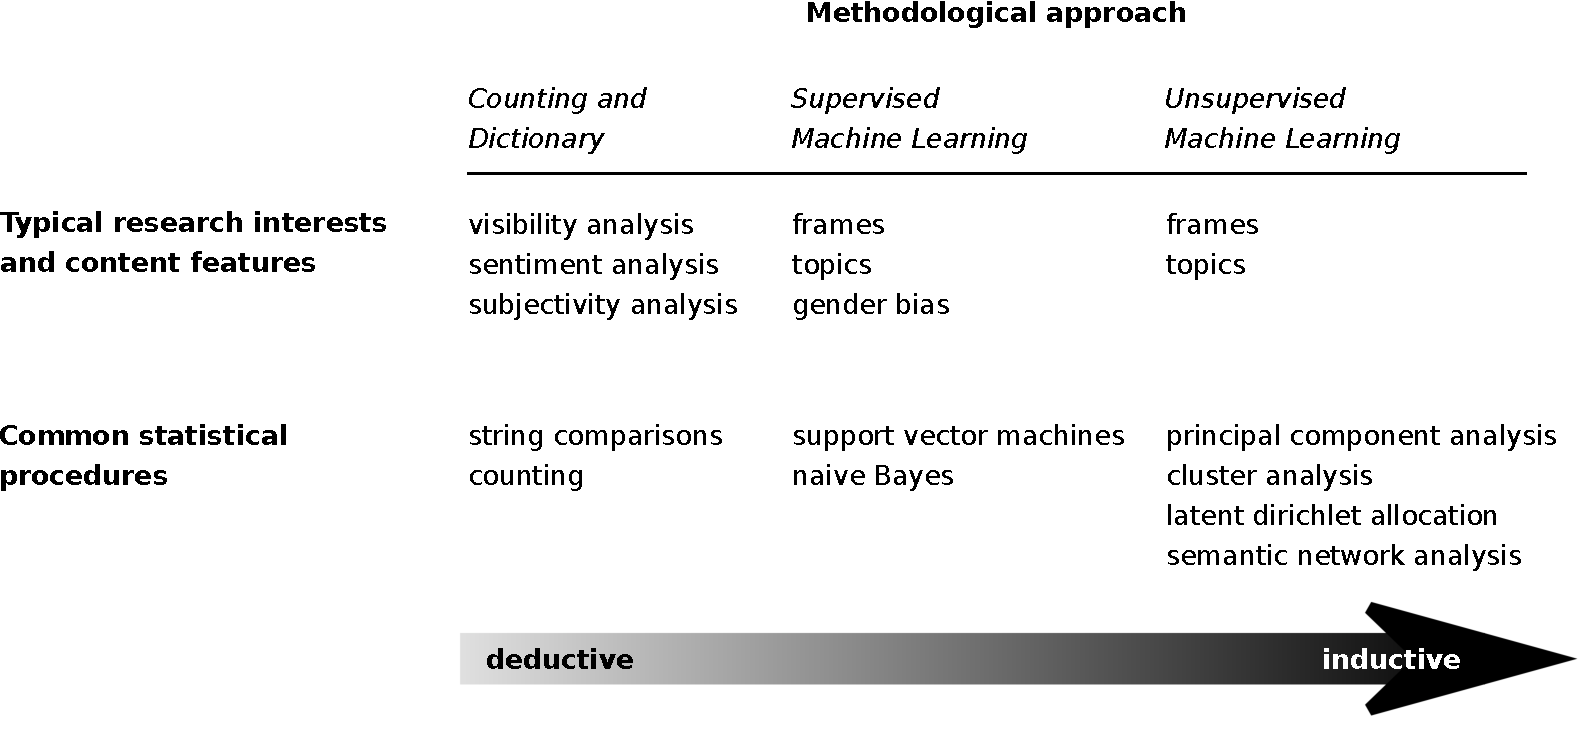
\includegraphics[width=\columnwidth,height=.8\paperheight,keepaspectratio]{boumanstrilling2016}}
\end{frame}

\begin{frame}{Bottom-up vs. top-down}
\begin{block}{Bottom-up}
	\begin{itemize}
		\item Count most frequently occurring words 
		\item Maybe better: Count combinations of words $\Rightarrow$ Which words co-occur together?
	\end{itemize}
	We \emph{don't} specify what to look for in advance	
\end{block}

\onslide<2>{
	\begin{block}{Top-down}
		\begin{itemize}
			\item Count frequencies of pre-defined words
			\item Maybe better: patterns instead of words
		\end{itemize}
		We \emph{do} specify what to look for in advance	
	\end{block}
}

\end{frame}


\begin{frame}[fragile]{A simple bottom-up approach}

\begin{minted}[%
	breaklines,
	linenos,
	fontsize=\scriptsize,
	frame=single,
	xleftmargin=0pt,]
	{python}
from collections import Counter
texts = ["Communication in the Digital Society is a very very complex phenomenon", "I like to study it"]
bottom_up = []
for t in texts:
    bottom_up.append(Counter(t.lower().split()).most_common(3))
    print(bottom_up)
\end{minted}
\pause
This results in:
\begin{minted}[fontsize=\scriptsize]{python}
[('very', 2), ('Communication', 1), ('in', 1)]
[('I', 1), ('like', 1), ('to', 1)]
\end{minted}
\textcolor{red}{\footnotesize{\emph{Please note that you can also write this like:}}}
\pause
\begin{minted}[%
	breaklines,
	linenos,
	fontsize=\scriptsize,
	frame=single,
	xleftmargin=0pt,]
	{python}
bottom_up = [Counter(t.split()).most_common(3) for t  in texts]
\end{minted}
\begin{itemize}
	\tiny{
		\item This is \emph{exactly} the same, just shorter (and faster). 
		\item You do \emph{not} have to use list comprehensions, but it helps if you can read them. }
\end{itemize}

\end{frame}

\begin{frame}[fragile]{A simple top-down approach}
\begin{minted}[%
	breaklines,
	linenos,
	fontsize=\scriptsize,
	frame=single,
	xleftmargin=0pt,]
	{python}
texts = ["Communication in the Digital Society is a very very complex phenomenon", "I like to study it"]
features = ["communication", "digital", "study"]
for t in texts:
    print(f"\nAnalyzing '{t}':")
    for f in features:
        print(f"{f} occurs {t.lower().count(f)} times")
\end{minted}
\pause
\begin{minted}[fontsize=\tiny]{python}
Analyzing 'Communication in the Digital Society is a very very complex phenomenon':
communication occurs 1 times
digital occurs 1 times
study occurs 0 times
	
Analyzing 'I like to study it':
communication occurs 0 times
digital occurs 0 times
study occurs 1 times	
\end{minted}
\end{frame}

\question{When would you use which approach?}


\begin{frame}{Some considerations}
\begin{itemize}[<+->]
	\item Both can have a place in your workflow (e.g., bottom-up as first exploratory step)
	\item You have a clear theoretical expectation? Bottom-up makes little sense.
	\item But in any case: you need to transform your text into something ``countable''.
\end{itemize}
\end{frame}

\section{Unsupervised Machine Learning for Text Classification}


\begin{frame}{Supervised vs Unsupervised}
	\begin{columns}[t]
		\column{.5\textwidth}
		
		\begin{block}<1-4>{Supervised machine learning}
			You have a dataset with both predictor and outcome (independent and dependent variables; features and labels) --- a \emph{labeled} dataset.
			\onslide<2>{
				\footnotesize{Think of regression: You measured \texttt{x1}, \texttt{x2}, \texttt{x3} and you want to predict \texttt{y}, which you also measured}}
		\end{block}
		
		\column{.5\textwidth}
		
		\begin{block}<3->{Unsupervised machine learning}
			You have no labels. \onslide<4>{(\footnotesize{You did not measure \texttt{y})}}\\
			\onslide<5>{\textbf{You might already know \emph{some} techniques to figure out whether \texttt{x1}, \texttt{x2},\ldots \texttt{x\_i} co-occur} \begin{itemize}
					\item Principal Component Analysis (PCA) and Singular Value Decomposition (SVD)
					\item Cluster analysis
					\item Topic modelling (Non-negative matrix factorization and Latent Dirichlet Allocation)
					\item \ldots
			\end{itemize}}
		\end{block}
		
	\end{columns}
	
\end{frame}


\subsection{An introduction to LDA}

\begin{frame}{}
	Enter \textbf{topic modeling with Latent Dirichlet Allocation (LDA)}
\end{frame}


\begin{frame}{LDA, what's that?}
	\begin{block}{No mathematical details here, but the general idea}
		\begin{itemize}
			\item There are $k$ topics, $T_1$\ldots$T_k$
			\item Each document $D_i$ consists of a mixture of these topics, e.g.$80\% T_1, 15\% T_2, 0\% T_3, \ldots 5\% T_k $
			\item On the next level, each topic consists of a specific probability distribution of words
			\item Thus, based on the frequencies of words in $D_i$, one can infer its distribution of topics
			\item Note that LDA is a Bag-of-Words (BOW) approach
		\end{itemize}
	\end{block}
	
\end{frame}


\begin{frame}[fragile]{Doing a LDA in Python}
	We will use gensim \parencite{Rehurek10softwareframework} for this (make sure you have version >4.0)
	
	Let us assume you have a list of lists of documents called \texttt{texts}:
	\begin{minted}[%
		breaklines,
		linenos,
		fontsize=\tiny,
		frame=single,
		xleftmargin=0pt,]
		{python}
print(texts[0][:115])
	\end{minted}
	\pause
	which looks something like:
	\begin{minted}[%
		fontsize=\tiny,
		breaklines,]
		{python}
'Stop the presses: CNN covered some actual news yesterday when it reported on the story of medical kidnapping victim Alyssa Gilderhus at the Mayo Clinic. But was it actually InfoWars and FreeMartyG which publicly shamed CNN into doing this real journalism? Cue the Mission Impossible theme music for this one...\n\nThis mission, as we accepted it, began more than a year ago during the baby Charlie Gard medical kidnapping scandal in the UK and we thought that it had ended with an apparently unsuccessf'
	\end{minted}
	
	\tiny{{\v R}eh{\r u}{\v r}ek, R., \& Sojka, P. (2010). Software framework for topic modelling with large corpora. \emph{Proceedings of the LREC 2010 Workshop on New Challenges for NLP Frameworks}, pp. 45–50. Valletta, Malta: ELRA. }
\end{frame}

\begin{frame}[fragile]{Preprocessing}
	Your preprocessing steps and feature engineering decisions \emph{largely} affect your topics
	\begin{enumerate}
		\item<1-> You can apply 'manual' preprocessing steps \dots
		\item<2->\dots In isolation or combination with for example \texttt{tfidf} transformations
	\end{enumerate}
	\pause
	\pause
	\begin{minted}[%
		breaklines,
		linenos,
		fontsize=\tiny,
		frame=single,
		xleftmargin=0pt,]
		{python}
texts_clean = [text.lower() for text in texts]
texts_clean=[" ".join(text.split()) for text in texts_clean]  #remove dubble spaces
texts_clean = ["".join([l for l in text if l not in punctuation]) for text in texts_clean] #remove punctuaction
texts_clean[0][:500]
	\end{minted}
	\pause
	which looks something like:
	\begin{minted}[%
		breaklines,
		fontsize=\tiny,]
		{python}
'stop the presses cnn covered some actual news yesterday when it reported on the story of medical kidnapping victim alyssa gilderhus at the mayo clinic but was it actually infowars and freemartyg which publicly shamed cnn into doing this real journalism cue the mission impossible theme music for this one this mission as we accepted it began more than a year ago during the baby charlie gard medical kidnapping scandal in the uk and we thought that it had ended with an apparently unsuccessful april '
	\end{minted}
\end{frame}


\begin{frame}[fragile]{Preprocessing}
	Without \emph{stopword removal},  \emph{tfidf} transformation and/or \emph{pruning}, you topics will not be very informative.
	\pause
	\begin{minted}[%
		breaklines,
		linenos,
		fontsize=\tiny,
		frame=single,
		xleftmargin=0pt,]
		{python}
mystopwords = set(stopwords.words('english')) # use default NLTK stopword list; alternatively:
# mystopwords = set(open('mystopwordfile.txt').readlines())  #read stopword list from a textfile with one stopword per line
texts_clean = [" ".join(word for word in text.split() if word not in mystopwords) for text in texts_clean]
texts_clean[0][:500]
	\end{minted}
	\pause
	which looks something like:
	\begin{minted}[%
		breaklines,
		fontsize=\tiny,]
		{python}
'stop presses cnn covered actual news yesterday reported story medical kidnapping victim alyssa gilderhus mayo clinic actually infowars freemartyg publicly shamed cnn real journalism cue mission impossible theme music one mission accepted began year ago baby charlie gard medical kidnapping scandal uk thought ended apparently unsuccessful april fools joke cnn sure many recall charlie gard infant rare form otherwise notsorare condition mitochondrial disease story went viral made international news '
	\end{minted}
\end{frame}

\begin{frame}[fragile]{Tokenization}
	\texttt{gensim} expects a list of words (hence: \texttt{tokenize} your corpus)
	\pause
	\begin{minted}[%
		breaklines,
		linenos,
		fontsize=\tiny,
		frame=single,
		xleftmargin=0pt,]
		{python}
tokenized_texts_clean = [TreebankWordTokenizer().tokenize(text) for text in texts_clean ] # tokenize texts; convert all strings to a list of tokens
tokenized_texts_clean[0][:500]
	\end{minted}
	\pause
	which looks something like:
	\begin{minted}[%
		breaklines,
		fontsize=\tiny,]
		{python}
['stop',
'presses',
'cnn',
'covered',
'actual',
'news',
'yesterday',
'reported',
'story',
..
	\end{minted}
\end{frame}

\begin{frame}[fragile]{LDA implementation}
	\texttt{LDA} implementation
	\pause
	\begin{minted}[%
		breaklines,
		linenos,
		fontsize=\tiny,
		frame=single,
		xleftmargin=0pt,]
		{python}
raw_m1 = tokenized_texts_clean
		
# assign a token_id to each word
id2word_m1 = corpora.Dictionary(raw_m1)   
# represent each text by (token_id, token_count) tuples
ldacorpus_m1 = [id2word_m1.doc2bow(text) for text in raw_m1] 
		
#estimate the model
lda_m1 = models.LdaModel(ldacorpus_m1, id2word=id2word_m1, num_topics=10)
lda_m1.print_topics()
	\end{minted}
	\pause
	
	\begin{minted}[%
		breaklines,
		fontsize=\tiny,]
		{python}
[(0, '0.015*"trump" + 0.012*"said" + 0.006*"president" + 0.006*"people" + 0.004*"cnn" + 0.004*"us" + 0.004*"house" + 0.004*"news" + 0.003*"also" + 0.003*"twitter"'),
(1,'0.010*"said" + 0.008*"trump" + 0.004*"one" + 0.004*"people" + 0.004*"us" + 0.004*"president" + 0.004*"would" + 0.003*"media" + 0.003*"also" + 0.003*"new"'),
(2, '0.011*"trump" + 0.009*"said" + 0.007*"president" + 0.005*"would" + 0.004*"people" + 0.004*"us" + 0.003*"also" + 0.003*"like" + 0.003*"news" + 0.003*"state"'),
(3, '0.010*"trump" + 0.006*"president" + 0.005*"said" + 0.004*"would" + 0.004*"us" + 0.003*"also" + 0.003*"people" + 0.003*"media" + 0.003*"news" + 0.003*"one"'),
	\end{minted}
\end{frame}




\begin{frame}[fragile]{Visualization with pyldavis}
	\begin{minted}[%
		breaklines,
		linenos,
		fontsize=\tiny,
		frame=single,
		xleftmargin=0pt,]
		{python}
import pyLDAvis
import pyLDAvis.gensim_models as gensimvis
# first estiate gensim model, then:
vis_data = gensimvis.prepare(lda_m1,ldacorpus_m1,id2word_m1)
pyLDAvis.display(vis_data)
	\end{minted}
	\makebox[\linewidth]{
		\includegraphics[width=\paperwidth,height=.5\paperheight,keepaspectratio]{../pictures/lda}}
\end{frame}

\iffalse
\begin{frame}{Visualization with pyldavis}
	Short note about the $\lambda$ setting:
	
	It influences the ordering of the words in pyldavis.
	
	\begin{quote}
		``For $\lambda = 1$, the ordering of the top words is equal to the ordering of the standard conditional word probabilities. For $\lambda$ close to zero, the most specific words of the topic will lead the list of top words. In their case study, Sievert and Shirley (2014, p. 67) found the best interpretability of topics using a  $\lambda$-value close to .6, which we adopted for our own case'' (Maier et al., 2018, p.~107)
	\end{quote}
	
	
	\tiny{Maier, D., Waldherr, A., Miltner, P., Wiedemann, G., Niekler, A., Keinert, A., \ldots Adam, S. (2018). Applying LDA Topic Modeling in Communication Research: Toward a Valid and Reliable Methodology. \textit{Communication Methods and Measures, 12}(2--3), 93--118. doi:10.1080/19312458.2018.1430754}
\end{frame}
\fi


\subsection{Choosing the best (or a good) topic model}

\begin{frame}{Choosing the best (or a good) topic model}
	\begin{itemize}
		\item There is no single best solution (e.g., do you want more coarse of fine-grained topics?)
		\item Non-deterministic
		\item Very sensitive to preprocessing choices
		\item Interplay of both metrics and (qualitative) interpretability 
	\end{itemize}
	
	See for more elaborate guidance:
	
	\tiny{Maier, D., Waldherr, A., Miltner, P., Wiedemann, G., Niekler, A., Keinert, A., \ldots Adam, S. (2018). Applying LDA Topic Modeling in Communication Research: Toward a Valid and Reliable Methodology. \textit{Communication Methods and Measures, 12}(2--3), 93--118. doi:10.1080/19312458.2018.1430754}
	
\end{frame}



\begin{frame}{Evaluation metrics}
	\begin{block}{qualitative: human judgement}
		Observation and interpretation based: observe the top N words in your topic, and evaluate the quality of the coherence of the topic.  Can you identify words that do not belong to a topic?
	\end{block}
	
	\pause 
	\begin{block}{quantitative: coherence}
		\begin{itemize}
			\item mean coherence of the whole model: attempts to quantify the interpretability
			\item coherence per topic: allows to get topics that are most likely to be coherently interpreted (\texttt{.top\_topics()})
		\end{itemize}
	\end{block}
	
\end{frame}


\begin{frame}{So, how do we do this?}
	\begin{itemize}[<+->]
		\item Estimate multiple models, store the metrics for each model, and then compare them (numerically, or by plotting)
		\item Idea: We select some candidate models, and then look whether they can be interpreted.
		\item But what can we tune?
	\end{itemize}
\end{frame}


\begin{frame}{Choosing $k$: How many topics do we want?}
	\begin{itemize}
		\item Typical values: $10<k<200$
		\item Too low: losing nuance, so broad it becomes meaningless
		\item Too high: picks up tiny pecularities instead of finding general patterns
		\item There is no inherent ordering of topics
		\item We can throw away or merge topics later, so if out of $k=50$ topics 5 are not interpretable and a couple of others overlap, it still may be a good model
	\end{itemize}
\end{frame}


\begin{frame}[fragile]{Choosing $\alpha$: how sparse should the document-topic distribution $\theta$ be?}
	\begin{itemize}
		\item The higher $\alpha$, the more topics per document 
		\item Default: $1/k$
		\item But: We can explicitly change it, or -- really cool -- even learn $\alpha$ from the data (\texttt{alpha = "auto"})
	\end{itemize}
	
	\pause 
	
	
	
	
	\begin{minted}[%
		breaklines,
		linenos,
		fontsize=\tiny,
		frame=single,
		xleftmargin=0pt,]
		{python}
mylda =LdaModel(corpus=tfidfcorpus[ldacorpus], id2word=id2word, num_topics=50, alpha='auto', passes=10)
	\end{minted}
	
\end{frame}


\iffalse
\begin{frame}{Choosing $\eta$: how sparse should the topic-word distribution $\lambda$ be?}
	\begin{itemize}
		\item Can be used to boost specific words
		\item Can also be learned from the data 
	\end{itemize}
	
	\pause
Takeaway: Even though you can do \texttt{eta="auto"}, this usually does not help you much.
	
\end{frame}
Takeaway: It takes longer, but you probably want to learn alpha from the data, using multiple passes:
\fi

% \subsection{Drawbacks of LDA topic models}


\subsection{Using topic models}

\begin{frame}{Using topic models}
	
You got your model -- what now?
	
	\begin{enumerate}
		\item Assign topic scores to documents
		\item Label topics
		\item Merge topics, throw away boilerplate topics and similar (manually, or aided by cluster analysis)
		\item Compare topics between, e.g., outlets
		\item or do some time-series analysis.
	\end{enumerate}
	
	
	Example:
	\tiny{Tsur, O., Calacci, D., \& Lazer, D. (2015). A Frame of Mind: Using Statistical Models for Detection of Framing and Agenda Setting Campaigns. \textit{Proceedings of the 53rd Annual Meeting of the Association for Computational Linguistics and the 7th International Joint Conference on Natural Language Processing} (pp. 1629–1638).}
	
\end{frame}


\begin{frame}[plain]
	
	\begin{block}{Try it out yourself..}
		\footnotesize
		\begin{itemize}
			\item Work through the example notebook on LDA: \url{https://github.com/uvacw/teaching-bdaca/blob/main/6ec-course/week07/exercises/topic-modelling.ipynb}
			\item \emph{Other resources}: 
			\url{https://github.com/uvacw/teaching-bdaca/blob/main/12ec-course/week10/lda.ipynb} \\
			\url{https://github.com/annekroon/gesis-machine-learning/blob/main/day3/excercise-afternoon/lda.ipynb}
		\end{itemize}
	\end{block}
	
\end{frame}



\section{Supervised Machine Learning for Text Classification}




\subsection{You have done it before!}
\begin{frame}{You have done it before!}
	\begin{block}{Regression}<2->
		\begin{enumerate}
			\item<3-> Based on your data, you estimate some regression equation 	$y_i = \alpha + \beta_1 x_{i1} + \cdots + \beta_p x_{ip} + \varepsilon_i$
			\item<4-> Even if you have some \emph{new unseen data}, you can estimate your expected outcome $\hat{y}$!
			\item<5-> Example: You estimated a regression equation where $y$ is newspaper reading in days/week: $y = -.8 + .4 \times man + .08 \times age$
			\item<6-> You could now calculate $\hat{y}$ for a man of 20 years and a woman of 40 years -- \emph{even if no such person exists in your dataset}: \\
			$\hat{y}_{man20} = -.8 + .4 \times 1 + .08 \times 20 = 1.2$ \\
			$\hat{y}_{woman40} = -.8 + .4 \times 0 + .08 \times 40 = 2.4$
		\end{enumerate}
	\end{block}	
	
\end{frame}



\begin{frame}{}
	\huge{This is\\ Supervised Machine Learning!}
\end{frame}

\begin{frame}{\ldots but\ldots}
	\begin{itemize}
		\item<1-> We will only use \emph{half} {\tiny{(or another fraction)}} of our data to estimate the model, so that we can use the other half to check if our predictions match the manual coding (``labeled data'',``annotated data'' in SML-lingo)
		\begin{itemize}
			\item<2->e.g., 2000 labeled cases, 1000 for training, 1000 for testing --- if successful, run on 100,000 unlabeled cases
		\end{itemize}
		\item<3-> We use many more independent variables (``features'')
		\item<4-> Typically, IVs are word frequencies (often weighted, e.g. tf$\times$idf) ($\Rightarrow$BOW-representation)
	\end{itemize}
\end{frame}


\subsection{From regression to classification}

\begin{frame}[standout]
	In the machine learning world, predicting some continous value is referred to as a \textcolor{orange}{regression} task. If we want to predict a binary or categorical variable, we call it a \textcolor{orange}{classification} task.
	
	(quite confusingly, even if we use a logistic regression for the latter)
\end{frame}


\begin{frame}{Classification tasks}
	For many computational approaches, we are actually not that interested in predicting a continous value. Typical questions include:
	\begin{itemize}
		\item Is this article about topic A, B, C, D, or E?
		\item Is this review positive or negative?
		\item Does this text contain frame F?
		\item Is this satire? 
		\item Is this misinformation?
		\item Given past behavior, can I predict the next click?
	\end{itemize}
\end{frame}



\begin{frame}[plain]
	\begin{columns}[]
		\column{.5\textwidth}
		
		{\tiny{http://commons.wikimedia.org/wiki/File:Precisionrecall.svg}}
		\makebox[\linewidth]{
			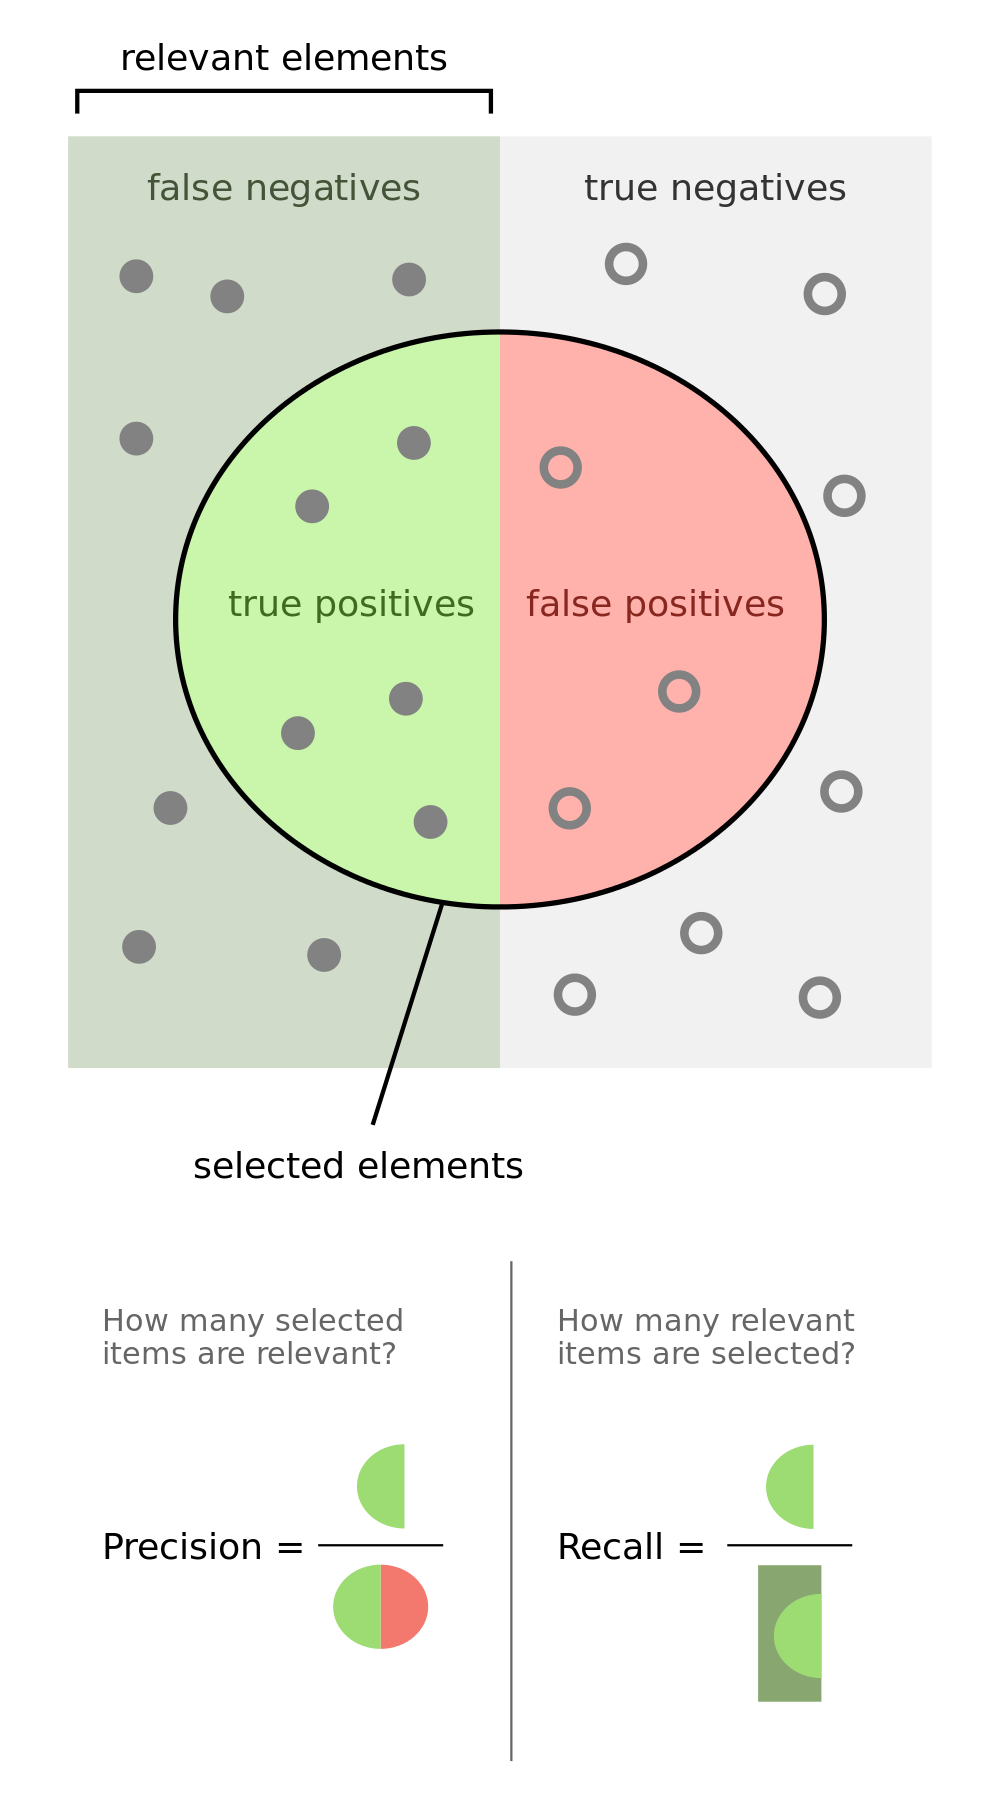
\includegraphics[width=\paperwidth,height=\paperheight,keepaspectratio]{../../resources/img/precisionrecall.png}}
		
		\column{.5\textwidth}
		\begin{block}{Some measures}
			\begin{itemize}
				\item Accuracy
				\item Recall
				\item Precision
				\item $\text{F1}=2\cdot \frac{\text{precision}\cdot \text{recall}}{\text{precision}+\text{recall}}$
				\item AUC (Area under curve) $[0,1]$, $0.5=$ random guessing
			\end{itemize}
		\end{block}
		
		
	\end{columns}
	
\end{frame}





\begin{frame}{Different classification algorithms}
	
	\begin{itemize}[<+->]
		\item It is an empirical question which one works best
		\item We typically try several ones and select the best
		\item (remember: we have a test dataset that we did \emph{not} use to train the model, so that we can assess how well it predicts the test labels based on the test features)
	\end{itemize}
	(to make it easier, imagine a binary classfication ("positive"/"negative"), but it doesn't really matter whether there are two or more labels)
\end{frame}




\begin{frame}{Dictionary-based approaches for text classification}
	\begin{columns}[t]
		\column{.5\textwidth}
		\begin{block}{good for}
			\begin{itemize}
				\item distinct, manifest things (names of organizations, pronouns, swearwords (?), \ldots)
				\item little room for interpretation/misunderstandings etc.
				\item ``must-be-explainable-to-a-five-year-old''
			\end{itemize}
			\pause
		\end{block}
		\column{.5\textwidth}
		\begin{alertblock}{bad for}
			\begin{itemize}
				\item latent constructs and concepts
				\item implicit things
			\end{itemize}
			\pause
			Hence, \emph{not} state-of-the-art for
			\begin{itemize}
				\item topics
				\item frames
				\item sentiment
			\end{itemize}
		\end{alertblock}
	\end{columns}
\end{frame}



\begin{frame}[standout]
	SML is no panacea, but the most promising approach to analyzing large quantities of texts. Don't believe off-the-shelf packages that claim to do the work for you.
	(For small datasets, just do it by hand.)
\end{frame}




\subsection{Diving into SML}


\subsection{An implementation}

\begin{frame}[fragile]{An implementation}
	Let's say we have a list of tuples with movie reviews and their rating:
	\begin{lstlisting}
reviews=[("This is a great movie",1),("Bad movie",-1), ... ...]
	\end{lstlisting}
	And a second list with an identical structure:
	\begin{lstlisting}
test=[("Not that good",-1),("Nice film",1), ... ...]
	\end{lstlisting}
Both are drawn from the same population, it is pure chance whether a specific review is on the one list or the other.\\
\tiny{Based on an example from \url{http://blog.dataquest.io/blog/naive-bayes-movies/}}
\end{frame}


\begin{frame}[fragile]{Training a A Naïve Bayes Classifier}
	\begin{minted}{python}
from sklearn.naive_bayes import MultinomialNB
from sklearn.feature_extraction.text import CountVectorizer
from sklearn import metrics
		
# This is just an efficient way of computing word counts
vectorizer = CountVectorizer(stop_words='english')
train_features = vectorizer.fit_transform([r[0] for r in reviews])
test_features = vectorizer.transform([r[0] for r in test])
		
# Fit a naive bayes model to the training data.
nb = MultinomialNB()
nb.fit(train_features, [r[1] for r in reviews])
		
# Now we can use the model to predict classifications for our test features.
predictions = nb.predict(test_features)
actual=[r[1] for r in test]
		
print("Precision: {0}".format(metrics.precision_score(actual, predictions, pos_label=1, labels = [-1,1])))
print("Recall: {0}".format(metrics.recall_score(actual, predictions, pos_label=1, labels = [-1,1])))
	\end{minted}
\end{frame}


\begin{frame}{And it works!}
	Using 50,000 IMDB movies that are classified as either negative or positive,
	\begin{itemize}
		\item I created a list with 25,000 training tuples and another one with 25,000 test tuples and
		\item trained a classifier
		\item with precision and recall values $>.80$
	\end{itemize}
	~\\
	\tiny{Dataset obtained from \url{http://ai.stanford.edu/~amaas/data/sentiment}, Maas, A.L., Daly, R.E., Pham, P.T., Huang, D., Ng, A.Y., \& Potts, C. (2011). Learning word vectors for sentiment analysis. \emph{49th Annual Meeting of the Association for Computational Linguistics (ACL 2011)}
	}
	
\end{frame}

\begin{frame}[fragile]{Playing around with new data}
	\begin{minted}{python}
newdata=vectorizer.transform(["What a crappy movie! It sucks!", "This is awsome. I liked this movie a lot, fantastic actors","I would not recomment it to anyone.", "Enjoyed it a lot"])
predictions = nb.predict(newdata)
print(predictions)
	\end{minted}
	This returns, as you would expect and hope:
	\begin{lstlisting} 
[-1  1 -1  1]
	\end{lstlisting}
	
	
\end{frame}

\begin{frame}{But we can do even better}
	We can use different vectorizers and different classifiers.
\end{frame}


\subsection{Classifiers}


\begin{frame}{Different classifiers}
	Typical options in a nutshell:
	\begin{itemize}
		\item Na\"ive Bayes
		\item Logistic Regression
		\item Support Vector Machine (SVM/SVC)
		\item Random forests
	\end{itemize}
\end{frame}





\begin{frame}{Which one would you (not) use for which purpose?}
	\makebox[\linewidth]{
		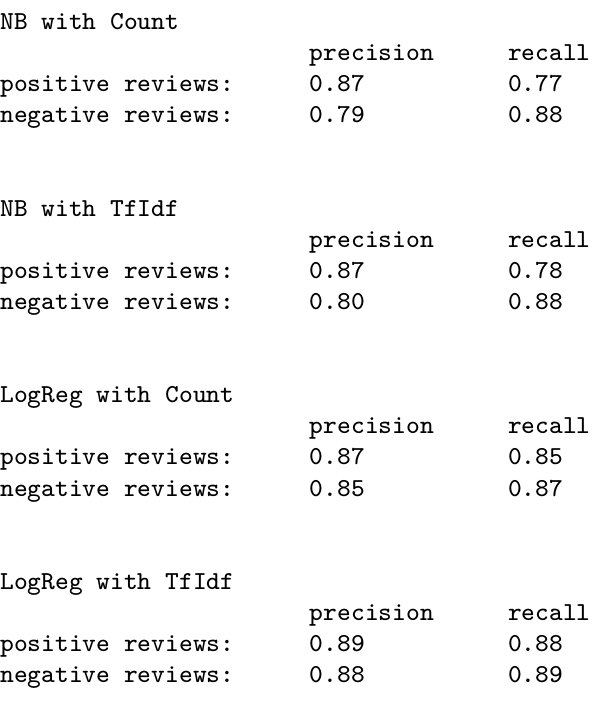
\includegraphics[width=\paperwidth,height=.8\paperheight,keepaspectratio]{imdbsml}}
\end{frame}




\section{Summing up}


\begin{frame}{What \emph{is} our fitted classifier again?}
	Essentially, just a formula 
	
	$$p = \frac{1}{1 + e^{-(\beta_0 + \beta_1 x_1 + \beta_2 x_2 + \ldots + \beta_n x_n)}}$$
	
	where $\beta_0$ is an intercept\footnote{Machine Learning people sometimes call the intercept ``bias'' (yes, I know, that's confusing)}, $\beta_1$ a coefficient for the frequency (or tf$\cdot$ idf score) of some word, $\beta_2$ a coefficient some other word.
	
	If our fitted \emph{vectorizer} contains 5,000 words, we thus have 5,001 coefficients.
	
	\tiny{(for logistic regression in this case, but same argument applies to other classifiers as well)}
	
\end{frame}

\question{But isn't that then essentially very much like a dictionary, except that the words have different weights?}


\begin{frame}{In some sense, yes.}
	\begin{itemize}
		\item But we don't pretend that we can construct the dictionary \emph{a priori}.
		\item It's specifically tailored to our use-case.
		\item The weights are \emph{really} essential here.
	\end{itemize}
	
	\pause
	We \emph{could} print all coefficients-word pairs, but probably it's enough to just look at those with the largest absolute value:
\end{frame}



\begin{frame}{ELI5}
	\makebox[\linewidth]{
		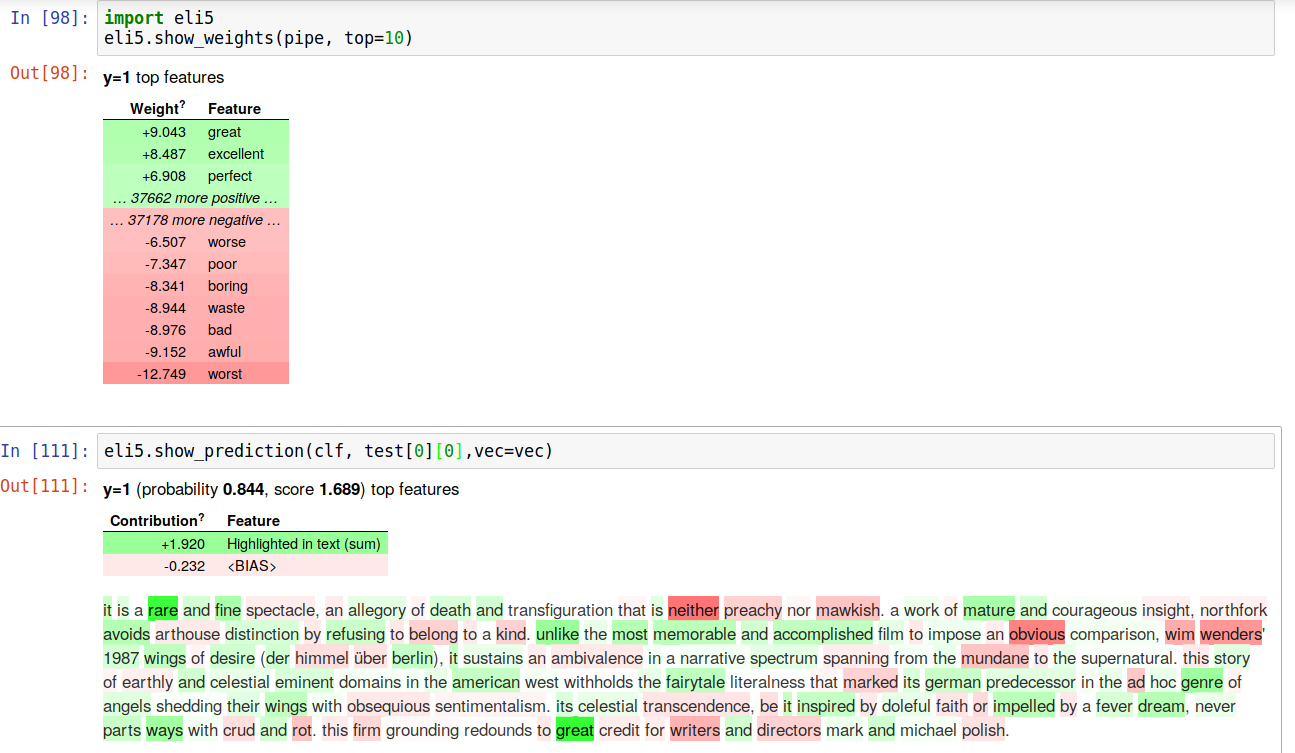
\includegraphics[width=\paperwidth,height=.8\paperheight,keepaspectratio]{eli5}}
\end{frame}

\begin{frame}{ELI5}
	\begin{itemize}
		\item Inspecting \emph{all} coefficients of a ML model usually doesn't make much sense
		\item But that does not mean that we cannot understand how the model makes its predictions
		\item We can look at the most important coefficients
		\item We can look which words in a given text contributed most to its classfication
	\end{itemize}
\end{frame}




\begin{frame}{But have we solved all problems of dictionaries?}
	No.
	
	For instance, the negation and/or intensifier problem.
	
	Possible approaches
	\begin{itemize}
		\item $n$-grams as features
		\item preprocessing (?)
		\item deep learning 
		\item \ldots
	\end{itemize}
	\pause
	
	$\Rightarrow$ \textbf{But ultimately, it's just an empirical question how big the problem is!}
	
	
\end{frame}


\subsection{A note on the input data}

\begin{frame}{The input scikit-learn expects}
	A training dataset consisting of:
	\begin{enumerate}
		\item an array (e.g., a list) of labels (\texttt{y\_train})
		\item a corresponding array (e.g., a list) of feature vectors (\texttt{X\_train})
	\end{enumerate}
	
	A test dataset consisting of:
	\begin{enumerate}
		\item an array (e.g., a list) of labels (\texttt{y\_test})
		\item a corresponding array (e.g., a list) of feature vectors (\texttt{X\_test})
	\end{enumerate}
	
	The feature vectors can be created via a \textit{vectorizer}, but could in principle also just be lists themselves.
	
	We use a lowercase \texttt{y} because it is a onedimensional vector, and an uppercase \texttt{X} because it is a two-dimensional matrix.
\end{frame}


\begin{frame}{The input scikit-learn expects}
	\begin{itemize}
		\item \textbf{It does not matter \emph{how} you create \texttt{y} and \texttt{X}!}
		\item Getting data into the right shape can be as much work (or more) as training the classifier itself
	\end{itemize}
	\pause
	Typical techniques:
	\begin{itemize}
		\item Reading text files from folders into lists of strings (looping over folder contents)
		\item Reading from csv file either directly into lists (\texttt{csv} module) or via pandas
		\item List comprehension to restructure or process data
		\item Potentially, you need to split into train and test dataset yourself (with slicing, or  with scikit-learn itself)
	\end{itemize}
\end{frame}


\begin{frame}{Looking forward: Beyond classic SML}
Note that classic SML is still based on word frequencies with weights (and hence cannot solve all problems we started off with). State-of-the art approaches like deep learning and transformers address this issue -- but that's for another time.
	
\end{frame}


\question{Any questions?}

\section{Next steps}

\begin{frame}[standout]
Thursday: time for your individual questions about the final project. 

I prepared exercises to work on \emph{during} the Thursday meeting (alone or in teams):
\large{\url{https://github.com/uvacw/teaching-bdaca/blob/main/6ec-course/week07/exercises/}}
\end{frame}





\begin{frame}[allowframebreaks,plain]
	\printbibliography
\end{frame}



\end{document}
